%\documentclass{beamer}
%\documentclass[notes=only]{beamer}   % only notes
\documentclass{beamer}              % only frames

\usetheme{simple}

\usepackage{lmodern}
\usepackage[scale=2]{ccicons}
\usepackage[T2A]{fontenc}
\usepackage[utf8]{inputenc}  
\usepackage[russian]{babel}
\usepackage{listings}
\usepackage{geometry}
\usepackage{marginnote}
\usepackage{movie15}
  
% TODO: 
%   position adjustement
%   change colours
%       

% Watermark background (simple theme)

%\setwatermark[hoffset=2cm,voffset=1,5cm]{
\includegraphics[height=8cm]{img/watermark1.png}}
\setwatermark{
\includegraphics[height=9cm]{img/watermark1.png}}


\title{Поиск программ для ПЛИС с помощью профилирования и эмуляции}
\subtitle{}
\date{\today}
\author{Баглий Антон}
\institute{\url{sfedu.ru}}

\begin{document}

\maketitle


\begin{frame}{поиск частей программ для отображения на ПЛИС}
  \framesubtitle{}
   
  \begin{columns}
    \column{.7\textwidth}
      \begin{itemize}
        \item Программы (или циклы), которые нужно ускорить
        \item Схемы для которых поместятся на ПЛИС
        \item Схемы для которых эффективно используют ресурсы
        \item Которые получат достаточное ускорение (с учетом памяти и т.п.)
      \end{itemize}

    \column{.3\textwidth}
      \begin{block}{В общем}
         Множество конфликтующих требований и факторов, влияющих на производительность
      \end{block}
  \end{columns}		  
\end{frame}

\begin{frame}[fragile]
\frametitle{Метрики кода и поверхностный статический анализ}
  \framesubtitle{Может ли это работать}
  \begin{columns}
    \column{.2\textwidth}
      \begin{itemize}
        \item Быстро работает
        \item Легко реализовать
      \end{itemize}
      
      \begin{block}{Поверхностный анализ}
         Тяжело получить хороший результат. Возможно накопление базы для применения методов машинного обучения (комп. статистики)
      \end{block}

    \column{.8\textwidth}
      
      
% TODO: хороший пример      
\begin{lstlisting}[frame=single]
 for (int i = 0; i < N; i++) {
   for (int j = 0; j < M; j++) {
      A = A*2;
   }
 }
\end{lstlisting}
\label{clone_listing}
      
  \end{columns}
  
\end{frame}

\begin{frame}[fragile]
\frametitle{Статический анализ}
  \framesubtitle{}
  \begin{columns}
    \column{.2\textwidth}
        \begin{itemize}
            \item Анализ потока данных
            \item Граф вычислений
            \item Конвейеризуемые циклы
        \end{itemize}      


    \column{.8\textwidth}
 
      
 % TODO: граф зависимостей?     
 % или граф вычислений?
\begin{lstlisting}[frame=single]

}
\end{lstlisting}
\label{encode_listing}
      
  \end{columns}
  
\end{frame}

\begin{frame}[fragile]
\frametitle{Отображение программы на ПЛИС}
  \framesubtitle{с низкоуровневого языка}
  \begin{columns}
    \column{.8\textwidth}
        \begin{itemize}
            \item графы вычислений
            \item конечные автоматы
            \item ...
            \item RTL
        \end{itemize}      


    \column{.8\textwidth}

\begin{lstlisting}[frame=single]

}
\end{lstlisting}
\label{encode_listing}
      
  \end{columns}
  
\end{frame}

% turn off watermark
\setwatermark{}

\begin{frame}{Динамический анализ}
  \framesubtitle{Инструментирование, профилирование}
  %TODO: преимущества?
  %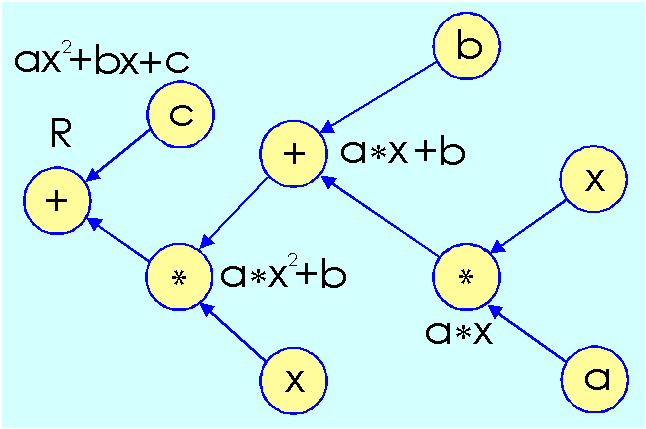
\includegraphics[height=8cm]{img/CalcGraphExample.png}
\end{frame}

\begin{frame}{Фазы выполнения программы}
  \framesubtitle{что это значит}
  %TODO: график из какого-то источника?
  
\end{frame}

\begin{frame}{Фазы выполнения программы}
  \framesubtitle{и части кода этой программы}
  Вопрос: как часто разные фазы работы соотвествуют разным циклам (функциям) или группам операторов?
  
  Ответ: 
  \begin{itemize}
      \item В некоторых примерах соответствуют
      \item Всегда можно придумать контрпример
  \end{itemize}
  % TODO: конкретные (не голословные) оценки, см. бенчмарки
  % TODO: визуализация на основе chstone?
  
\end{frame}

\begin{frame}{Выбор уровня представления программы для анализа}
  \framesubtitle{высокоуроевневое дерево или промежуточные код?}
  
  \begin{itemize}
      \item AST
      \item SSA
  \end{itemize}
  
\end{frame}

\begin{frame}{Эмуляция архитектуры}
  \framesubtitle{}
  
  \begin{itemize}
      \item Высокотоная эмуляция архитектуры процессора возможна
      \item Но только по полному описанию этой архитектуры
      \item что если мы хотим сделать эмулятор для очень грубой оценки времени работы программы?
      \item ПЛИС это не архитектура, а конструктор любой архитектуры
      \item но возможно составить грубую модель времени выполнения, которая будет отдаленно напоминать реконфигурируемую архитектуру обладающую определенными ресурсами
  \end{itemize}
  
\end{frame}

\begin{frame}{ПЛИС как конструктор вычислительного устройства}
  \framesubtitle{из более крупных блоков}
  
  \begin{itemize}
      \item IP-core
      \item тенденция к укрупнению блоков (не уножители и LUT, а целые DSP и др. готовые устройства) 
      \item возможно представить ресурсы ПЛИС как набор функциональных модулей (вычислителей) на которые отображаются вычисления в исходной программе
 \end{itemize}
  
\end{frame}

\begin{frame}{Скорость работы эмуляции архитектуры}
  \framesubtitle{}
  
  \begin{itemize}
      \item медленно
      \item точный анализ (например, анализ алиасов, анализ указателей) медленный
  \end{itemize}

\end{frame}

\begin{frame}{Вектор простых блоков}
  \framesubtitle{}
  
  \begin{itemize}
      \item Статистика по простым блокам, посещенным во время выполнения
      \item Позволяет статистически оценить поведение программы на тестовых данных
      \item Позволяет найти выборку простых блоков (и конкретные моменты во время работы), по которым можно прогнозировать время работы программы в целом
  \end{itemize}
  
\end{frame}


\begin{frame}{Simpoints и аналогичные алгоритмы}
  \framesubtitle{}
  
  \begin{itemize}
      \item Простой статистический метод выбора репрезентативных точек во время выполнения
      
  \end{itemize}
  
\end{frame}

\begin{frame}{Проект эмулятора}
  \framesubtitle{}
  
  \begin{itemize}
      \item набор функциональных модулей
      \item связи между ними
      \item оценка времени работы при интерпретации
  \end{itemize}
  
\end{frame}

\begin{frame}{Проект эмулятора - текущие результаты}
  \framesubtitle{}
  
  \begin{itemize}
      \item Прототип на LLVM
      \item Интерпретатор
  \end{itemize}
  
\end{frame}

\begin{frame}[allowframebreaks]
        \frametitle{References}
        \bibliographystyle{amsalpha}
        \bibliography{references.bib}
\end{frame}

\end{document}